\documentclass{article}

\input{../../../assets/settings/newcommand.tex}
\input{../../../assets/settings/usepackage.tex}
% \input{../../../assets/settings/quitarnumerossecciones.tex}

% \usepackage{nopageno} % Paquete para desactivar la numeración de páginas

\title{Memoria}
\author{KGNETE}
\date{\today}

\begin{document}

\maketitle

\chapter{Memoria}

\section{Objeto}
El objeto es justificar las soluciones adoptadas, su adecuación a la normativa legal aplicable y, conjuntamente
con los planos y el pliego de condiciones, describir de forma unívoca el objeto del Proyecto.

\section{Alcance}

Se genera la energia que se consume en la propia instalacion.

\section{Antecedentes}

Se trata de una ampliación de la instalacion receptora con una instalacion generadora de electricidad.

\section{Normas y referencias}

La instalación se realizará conforme a la normativa vigente, incluyendo pero no limitándose a:

\subsection{Disposiciones legales y normas aplicadas}

% \href{https://www.idae.es/sites/default/files/documentos/publicaciones_idae/2023_10_20_Guia_Autoconsumo_Ayuntamientos_v4.pdf}{Disposiciones legales y normas aplicadas}
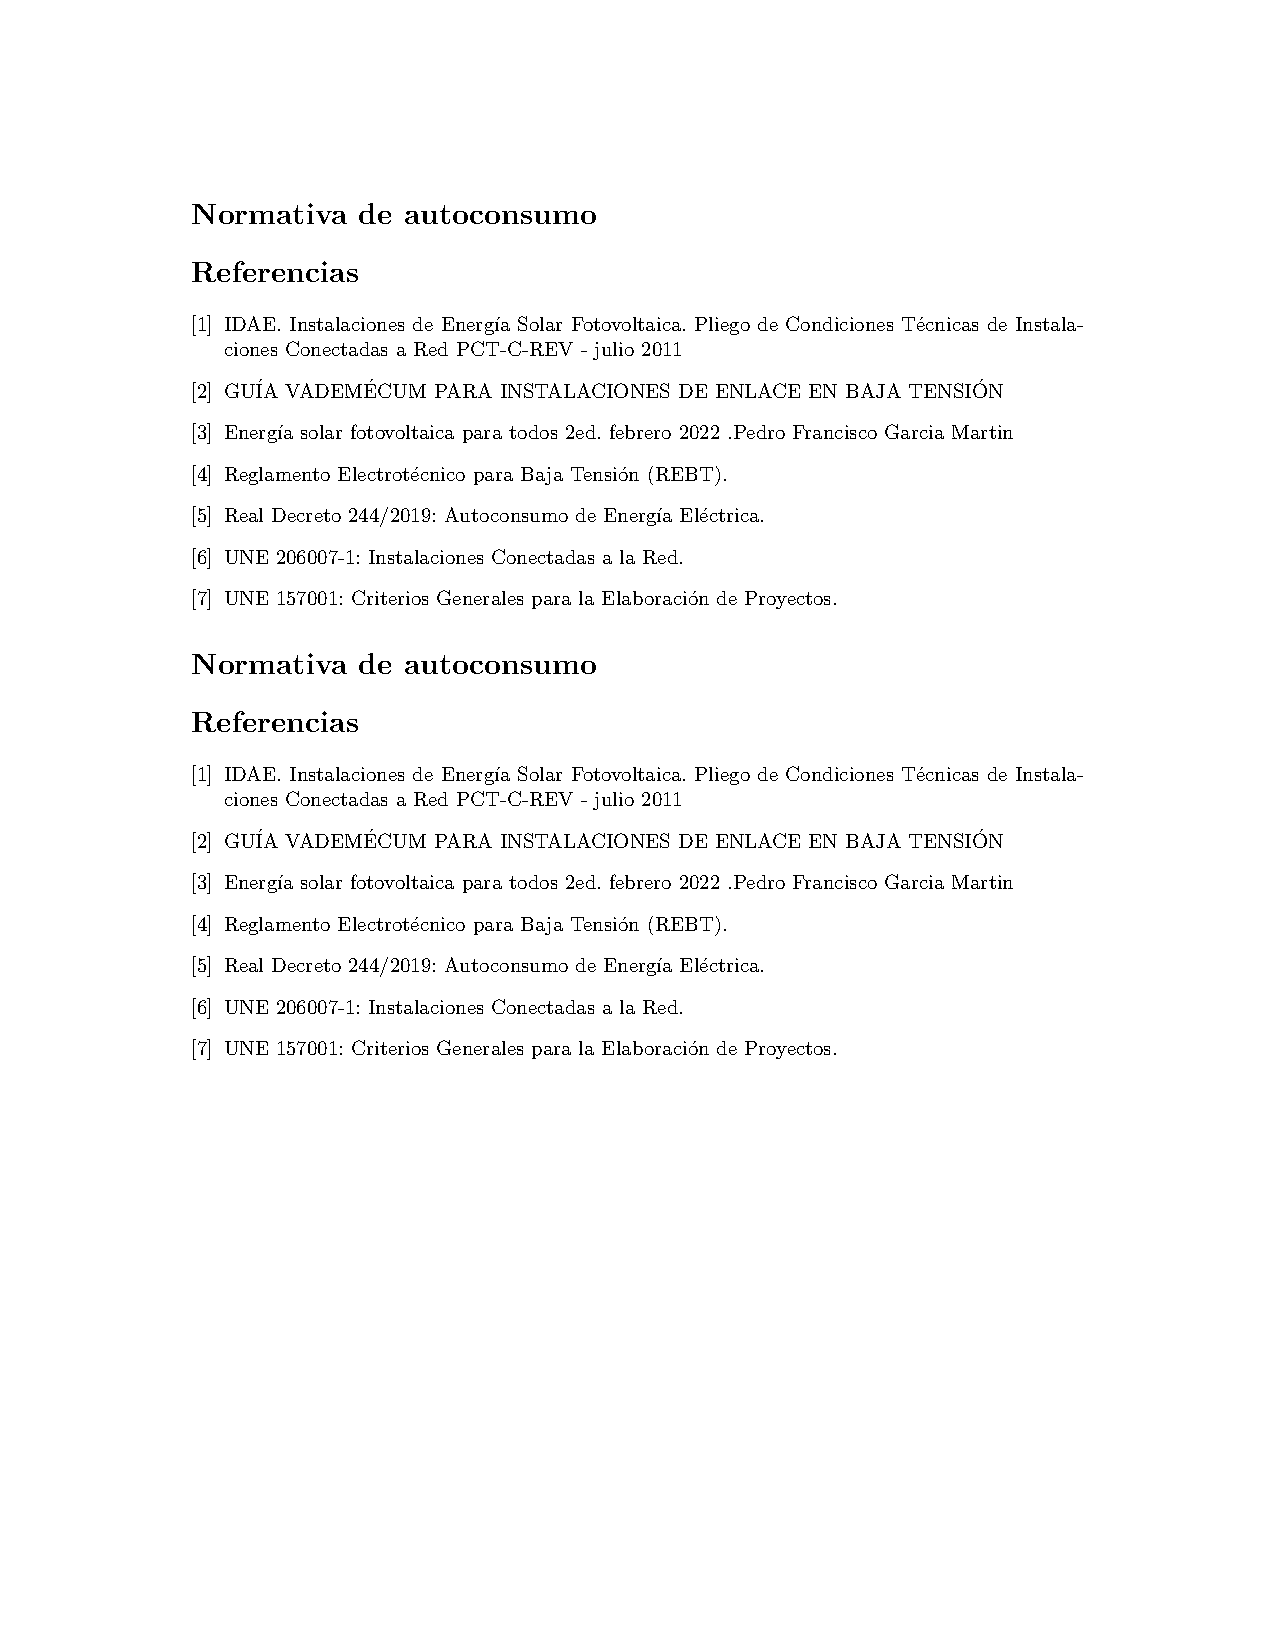
\includepdf[pages=-, pagecommand={\thispagestyle{fancy}}]{../DOCUMENTOS/Normativa Autoconsumo.pdf}


Las instalaciones de autoconsumo de cualquier tecnología de generación, están sometidas a la normativa eléctrica que les aplique en función de su potencia y de la conexión que realicen, bien en baja tensión (BT) o en alta tensión (AT).


En este apartado se describen los conceptos fundamentales extraídos de la normativa eléctrica y las principales autorizaciones que las instalaciones de autoconsumo deben obtener, puesto que dependen del tamaño de la instalación (en términos de potencia) y pueden servir de guía a los técnicos municipales para valorar su complejidad y la magnitud de las actuaciones que implican.

\subsubsection{Solicitud de acceso y conexión}

El acceso y conexión aparece regulado por el Real Decreto 1183/2020, de 29 de diciembre, de acceso y conexión a las redes de transporte y distribución de energía eléctrica.

El procedimiento a seguir queda regulado por el mismo Real Decreto y por la Circular 1/2021 de 20 de enero, de la Comisión Nacional de los Mercados y la Competencia, por la que se establece la metodología y condiciones del acceso y de la conexión a las redes de transporte y distribución de las instalaciones de producción de energía eléctrica.

Con este trámite, se solicita permiso para acceder a la red pública de transporte o distribución y se obtienen las condiciones en las que dicho acceso es posible y cómo y dónde deberá realizarse la conexión a la misma. Además, se obtienen la potencia que será posible conectar.

Este trámite incluye la presentación de garantías económicas por una cuantía equivalente a 40 €/kW de potencia que se solicita, y cuyo resguardo de presentación se deposita ante el órgano competente para otorgar la autorización de la instalación. La finalidad de la garantía será la obtención de la autorización de explotación.

Las instalaciones de autoconsumo SIN excedentes están exentas de realizar este trámite de acceso y conexión y, por tanto, tampoco tienen que presentar la garantía.

Las instalaciones de autoconsumo CON excedentes de potencia igual o inferior a 15 kW que se ubiquen en suelo urbanizado que cuente con las dotaciones y servicios requeridos por la legislación urbanística, también están exentas de realizar el trámite de acceso y conexión y por tanto tampoco deberán presentar la garantía.

El resto de instalaciones de autoconsumo CON excedentes siempre que sean de potencia igual o inferior a 100 kW, sí tendrán que realizar el trámite de acceso y conexión, pero no precisan aportar la garantía, salvo que estas instalaciones formen parte de una agrupación cuya potencia sea superior a 1 MW, de acuerdo con la definición de agrupación establecida en el artículo 7 del Real Decreto 413/2014, de 6 de junio. En el caso de que además sean de potencia inferior a 15kW podrán acogerse al procedimiento abreviado, cuyos plazos serían la mitad que en el procedimiento general.

Desde la aprobación del Real Decreto-ley 23/2020, de 23 de junio es posible que la potencia de acceso concedida sea inferior a la potencia que figura en la autorización administrativa. La capacidad de acceso será la potencia activa máxima que se le permite verter a la red a una instalación de generación de electricidad.

\subsubsection{Autorización administrativa}

La Ley 24/2013, de 26 de diciembre, del Sector Eléctrico regula el régimen de autorizaciones de las instalaciones de generación, incluidas las de autoconsumo, entre las que se incluyen:

- a) Autorización administrativa previa, que se tramitará con el anteproyecto de la instalación como documento técnico y, en su caso, conjuntamente con la evaluación de impacto ambiental, según lo dispuesto en la Ley 21/2013, de 9 de diciembre, de evaluación ambiental, y otorgará a la empresa autorizada el derecho a realizar una instalación concreta en determinadas condiciones.

- b) Autorización administrativa de construcción, que permite al titular realizar la construcción de la instalación cumpliendo los requisitos técnicos exigibles. Para solicitarla, el titular presentará un proyecto de ejecución junto con una declaración responsable que acredite el cumplimiento de la normativa que le sea de aplicación. La tramitación y resolución de autorizaciones definidas en los párrafos anteriores podrán efectuarse de manera consecutiva, coetánea o conjunta.

- c) Autorización de explotación, que permite, una vez ejecutado el proyecto, poner en tensión las instalaciones y proceder a su explotación.

El Real Decreto 1955/2000 en su artículo 111 exime de este trámite a las instalaciones de tensión inferior a 1kV. Adicionalmente, el Real Decreto 1699/2011 exime a las instalaciones de producción de energía eléctrica con potencia nominal no superior a 100 kW, conectadas directamente a una red de tensión no superior a 1 kV, ya sea de distribución o a la red interior de un consumidor.

\subsubsection{Reglamentos técnicos}

Ley 24/2013, de 26 de diciembre, del Sector Eléctrico, establece que las instalaciones de autoconsumo conectadas en baja tensión se ejecutarán de acuerdo con lo establecido en el Reglamento Electrotécnico de Baja Tensión (REBT) y sus Instrucciones Técnicas complementarias (ITC-BT). Según determina la ITC-BT-40, será admisible la conexión a BT de las instalaciones de  autoconsumo CON excedentes de hasta 100 kW y en todas las instalaciones de autoconsumo SIN excedentes.

Por esta razón, cualquier instalación de autoconsumo conectada a las redes de baja tensión contará con un Certificado de Instalación eléctrica (CIE) firmado por una empresa instaladora habilitada y debidamente diligenciado por el órgano competente de la comunidad autónoma, que asegurará que esta ha sido llevada a cabo en base a lo establecido en el REBT.

De acuerdo con el REBT, si la instalación tiene una potencia superior a 10 kW deberá disponer de un proyecto técnico firmado por técnico competente. Las instalaciones de menor potencia (hasta 10 kW) únicamente tienen obligación de disponer de una Memoria Técnica de Diseño (MTD) según el formato de la comunidad autónoma, firmada por la empresa instaladora habilitada.

En el caso de las instalaciones conectadas en alta tensión el reglamento aplicable será el Reglamento de Instalaciones Eléctricas de Alta Tensión (RAT) y sus Instrucciones Técnicas complementarias (ITC-RAT)

\subsubsection{Registro Administrativo de Autoconsumo (RADNE)}

El RD 244/2019 establece que todas las instalaciones de autoconsumo deberán estar registradas en el Registro Administrativo de Autoconsumo que es competencia de la Dirección General de Política Energética y Minas del Ministerio para la Transición Ecológica y el Reto Demográfico y que se encuentra regulado en el artículo 19 de dicho real decreto.

Las comunidades autónomas y las ciudades autónomas de Ceuta y Melilla pueden crear sus propios registros de autoconsumo de carácter autonómico, pero en cualquier caso deben proporcionar la información necesaria para la inscripción (descrita en el ANEXO II del RD 244/2019) al Ministerio.

Este paso administrativo es transparente para el consumidor y/o promotor de la instalación de autoconsumo ya que se realiza de oficio entre administraciones y resulta el último trámite en la legalización de una instalación de autoconsumo. Para obtener más información sobre la tramitación administrativa de las instalaciones de autoconsumo puede consultar la Guía Profesional de Tramitación del Autoconsumo disponible en <https://www.idae.es/>

\subsubsection{Ordenanzas urbanísticas}

\subsubsection{Autónomica}

Leyes de urbanismo y de ordenación del suelo.

\subsubsection{Municipal}

El municipio  establece tres tipos de trámites para estas autorizaciones:

- Licencia de obra.

- Declaración responsable de obra.
Normalmente se destina a aquellas actuaciones técnicamente sencillas y que no precisen
elementos estructurales, y que no supongan alteración del volumen, del uso principal de
las instalaciones y servicios de uso común o del número de viviendas y locales, ni afecten
a la composición exterior, a la estructura o a las condiciones de habitabilidad o seguridad.

- Comunicación previa a la ejecución de obra.
Normalmente pequeñas actuaciones y/o reformas.

La instalacion fotovoltaicas de autoconsumo se ubica en la cubierta de edificio ya existente, cumplen las características de sencillez técnica y no afectación a elementos estructurales del edificio. En ningún caso supone aumento de superficie habitable.

Estas características de las instalaciones de autoconsumo fotovoltaico sobre edificacion permite a los municipios la aplicación de procedimientos de declaración responsable o comunicación previa en la concesión de las licencias de obras.

Para la redacción del presente proyecto se han tenido en cuenta las normas y disposiciones legales (leyes, reglamentos, ordenanzas, nor-
mas de obligado cumplimiento por su inclusión en disposiciones legales, etc.)

% {excel2md.normativa()}


% \subsection{Programas de cálculo}

% - Excel

% - PHOTOVOLTAIC GEOGRAPHICAL INFORMATION SYSTEM (PVGIS)

% \subsection{Plan de gestión de la calidad aplicado durante la redacción del Proyecto}

% Los procesos específicos utilizados

% - Aseguramiento de la calidad del proceso
% Durante la ejecución del proyecto, se monitorean y evalúan continuamente los procesos para asegurarse de que se estén siguiendo según lo planeado. Esto implica revisar regularmente si se cumplen los estándares y realizar ajustes si es necesario.

% - Revisiones:
% Se llevan a cabo revisiones periódicas de las actividades y los productos entregables para identificar posibles problemas o desviaciones con respecto a los estándares de calidad establecidos.

% - Gestión de cambios:
% El control de cambios es esencial para asegurar la calidad. Cualquier cambio en los requisitos o en el alcance del proyecto debe ser gestionado cuidadosamente para evitar impactos negativos en la calidad

% - Pruebas y validación:
% Se realizan pruebas exhaustivas en todas las fases del proyecto para verificar que los productos cumplen con los requisitos y estándares de calidad establecidos. Esto puede incluir pruebas de funcionalidad, rendimiento, seguridad, entre otras.

% - Mejora continua:
% Después de la finalización del proyecto, se realiza una revisión exhaustiva para analizar lecciones aprendidas y identificar áreas de mejora. Esto alimenta el ciclo de mejora continua, permitiendo ajustes en los procesos para futuros proyectos.

% \subsection{Bibliografía}

% - Instalaciones solares fotovoltaicas 2ª edición , Miguel Moro Vallina, 21/2/2024

% - Configuración de instalaciones solares fotovoltaicas 2.ª edición 2022 , Julian Cantos Serrano, 7/7/2023
% % Para justificar las soluciones adoptadas en el Proyecto se han considerado de interes:

% % {o.Normativa{o.Normativa{'Tipo'} == 'Bibliografía'}.loc{:, 'Denominacion'}.dropna().reset_index(drop=True).to_markdown(headers={''*5})}

% \subsection{Otras referencias}

% - \href{https://www.idae.es/tecnologias/energias-renovables/oficina-de-autoconsumo/guias-tecnicas-sobre-autoconsumo}{Guías técnicas y Formación sobre autoconsumo,  IDAE}

% \section{ Definiciones y abreviaturas}

% % <!-- 
% % En este capítulo de la memoria se deben relacionar todas las definiciones, abreviaturas, etc. que se han utilizado y su significado. 
% % -->

% % {indice.abreviaturas()}

% \section{ Requisitos de diseño}

% <!-- 
% En este capítulo de la memoria se deben describir las bases y datos de partida que se derivan de:
%  el cliente,
%  el emplazamiento, y su entorno socio-económico y ambiental,
%  los estudios realizados encaminados a la definición de la solución adoptada,

%  las interfaces con otros sistemas o elementos externos al proyecto u otros que condicionan las soluciones técnicas del mismo.
%  -->

\section{ Análisis de soluciones}


\addcontentsline{toc}{subsection}{Disposicion de los paneles}
\includepdf[pages=-, pagecommand={\thispagestyle{fancy}}]{../ESTUDIOS/Disposicion de los paneles.pdf}


\addcontentsline{toc}{subsection}{Rentabilidad de una bateria}
\includepdf[pages=-, pagecommand={\thispagestyle{fancy}}]{../ESTUDIOS/Rentabilidad de una bateria.pdf}



\section{ Resultados Instalacion FV}

\addcontentsline{toc}{subsection}{Rentabilidad de una bateria}
\includepdf[pages=-, pagecommand={\thispagestyle{fancy}}]{../CALCULOS/Resultados Instalacion FV.pdf}



% - Las características definitorias de la instalación elegida, indicada enla tabla esta desarrolada en el apartado planos.

\subsection{Rendimiento de un sistema FV conectado a red (PVGIS)}
\includepdf{../../assets/varios/PVGIS.pdf}


\subsection{Analisis finaciero (SAM)}

\section{ Planificación}

En relación al proceso de materialización del Proyecto, se definen las etapas agrupadas segun la figura.

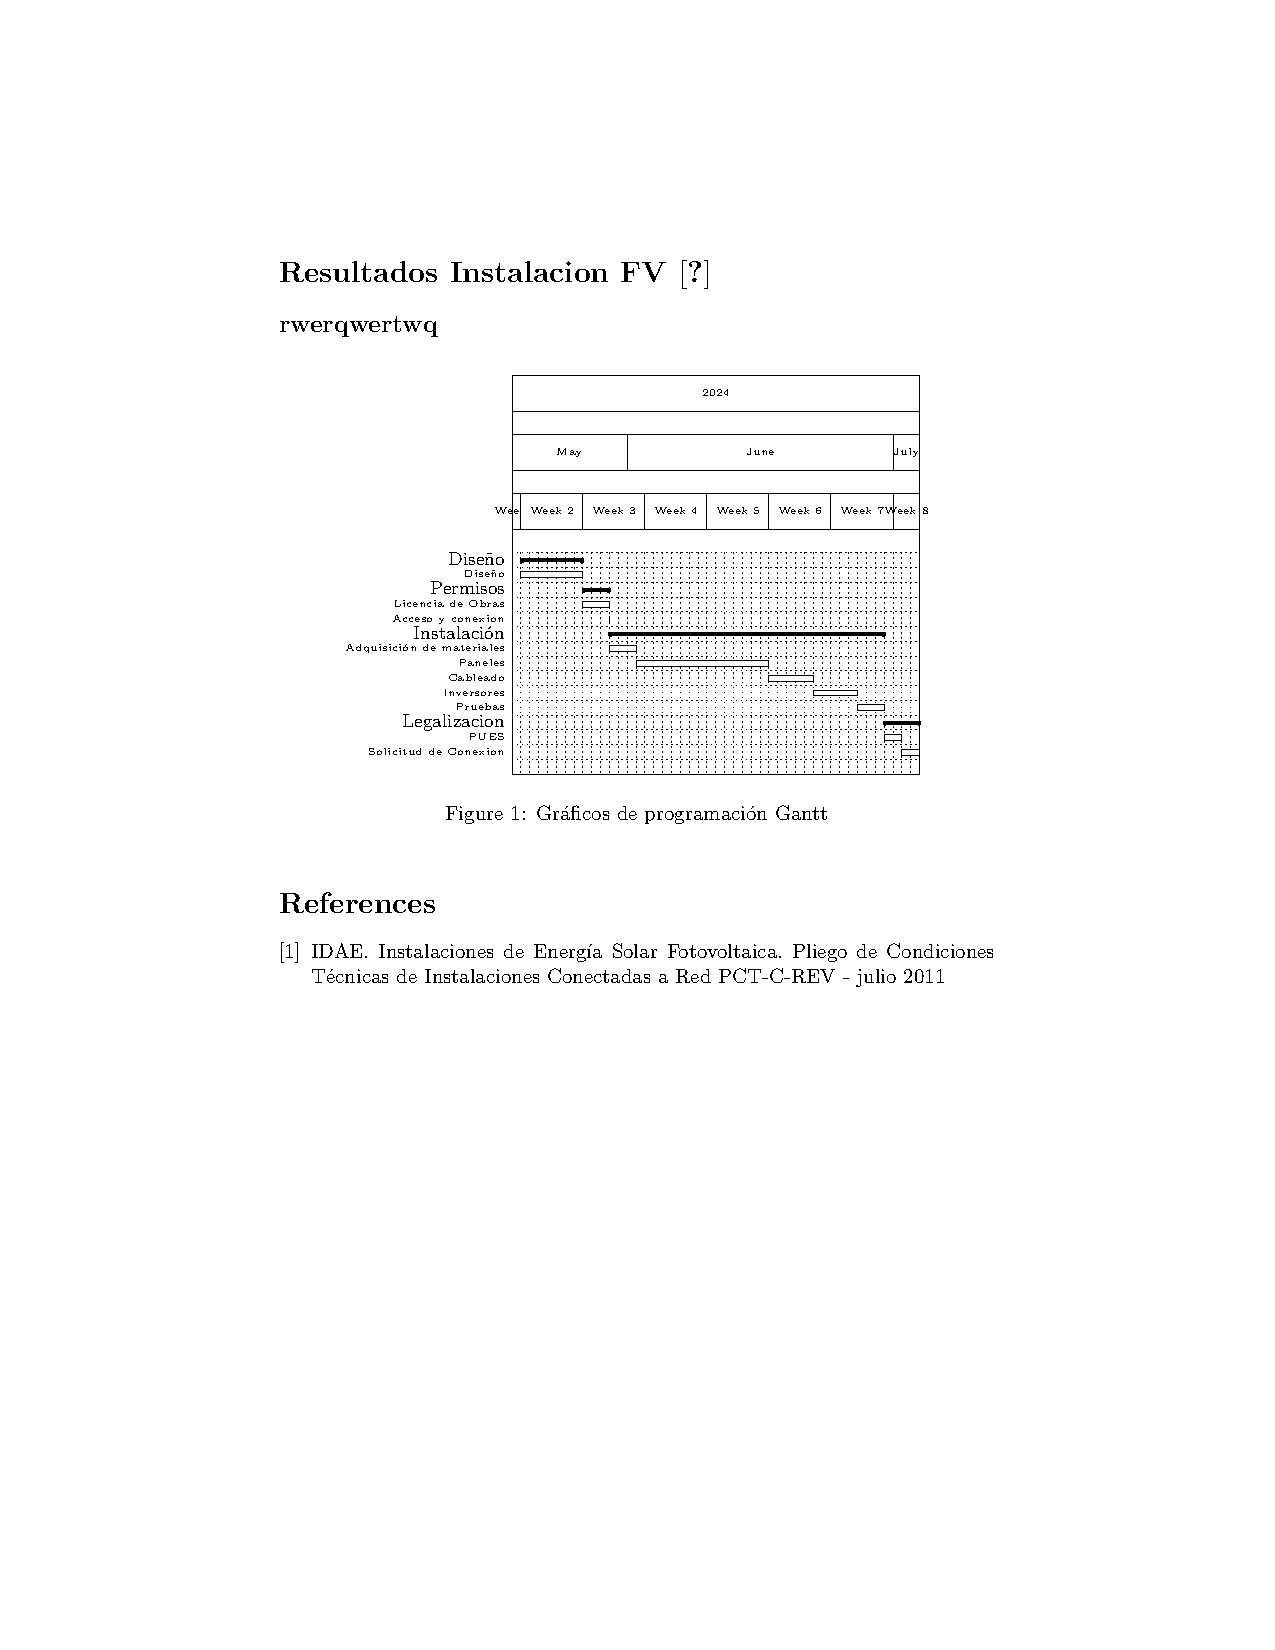
\includepdf[pages=-, pagecommand={\thispagestyle{fancy}}]{../DOCUMENTOS/Planificacion.pdf}

% {figltx.gantt()}

\section{ Orden de prioridad entre los documentos}

El orden de prioridad debe ser el siguiente:

1 Planos.

2 Pliego de condiciones.

3 Presupuesto.

4 Memoria.



\end{document}
